\chapter{Spiking Neural Networks~(SNNs)}
\label{cha:bkg}
Biological studies have obtained increasing knowledge about facts, functions and anatomy of the brain.
At the cellular level, the central nervous system consists of two types of cells: neurons, the elementary processing units, and glial cells, the structural and metabolic supporters. 
Here we focus on the neurons, since they connect to each other forming the path from neural circuit and network to behaviour and cognition of the brain.
The human brains contains around a hundred of billions ($10^11$) such processing units, and three more orders of magnitudes connections, that are about $10^3$ connections per neuron.
The special structures of neurons enable them to send signals rapidly and precisely to other cells through these connections.


\section{Biological Neural Components}
\subsection{Neuron}
	\begin{figure}[bt]
	\centering
	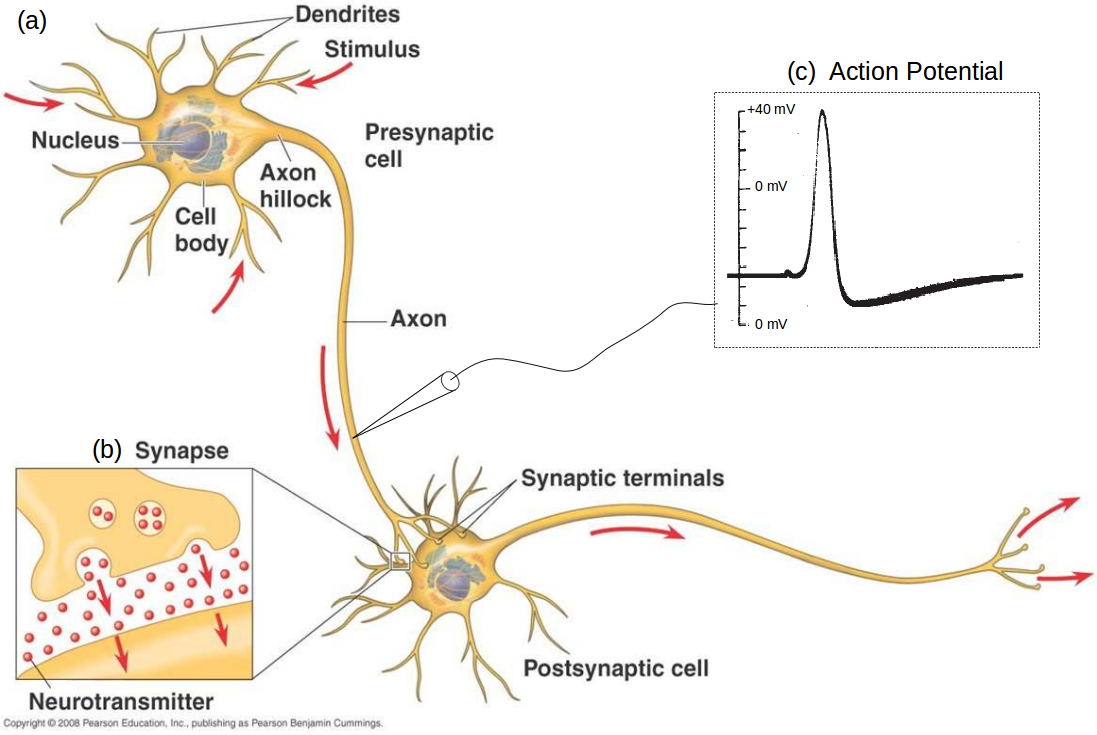
\includegraphics[width=0.98\textwidth]{pics_snn/neuron2.png}
	\caption{Two neurons connected by synapses. 
		A neuron mainly is composed of three functional parts: dendrites, the soma, and the axon. (a) A pre-synaptic cell connects to its post-synaptic cell through synapses~\cite{reece2011campbell}, see (b)~\cite{reece2011campbell}, and the neural signal, action potential see (c)~\cite{hodgkin1939action}, propagates along the red arrows. }
	\label{Fig:neuron_basic}
\end{figure}
A typical neuron consists of three functional parts: dendrites, a cell body (soma), and an axon, see Figure~\ref{Fig:neuron_basic}(a).
The dendrites of a neuron receive stimuli from other neurons which the dendrites project to, and transmit the neural signal to the neuron's soma.
The soma is the cell body of the neuron where nucleus locates at, and functions like a non-linear processor that it triggers an output signal when accumulated total input exceeds some threshold.
The output signal initiates from the axon hillock where the axon emerges from the soma, and then propagated through the axon to other neurons.
Most of the neurons contains only one axon, but it may connects to many neurons by branching out axon terminals. 


The signal delivery from a neuron to another occurs at the junction between these two neurons, which is called a synapse, see Figure~\ref{Fig:neuron_basic}(b).
The neurons can be seen as a pre-synaptic cell which sends the signal, and a post-synaptic cell which receives.

%Spiking neuron models can be divided into two major categories \cite{gernstbook} based on their level of abstraction: The conductance models and the threshold models.
%The conductance models simulate a lower level on the ion channels, while the threshold models represent a higher level of neuron abstraction where the threshold voltage is fixed and the neuron fires once the membrane potential reaches it.
%
%In general, Conductance-Based models have been derived from the Nobel prize winners (1963) Hodgkin and Huxley, based on the experiments that they performed on the giant axon squid \cite{hhmodel}.
%Spikes arriving at a LIF neuron cause a temporary flow of current into (excitatory synapse) or out of (inhibitory synapse) the neuron, modelling the behaviour of synapses in biological neurons.
%The LIF neuron sums up this current over time, accumulating charge which gradually leaks away.
%If the membrane potential in the neuron reaches a certain threshold, it produces a spike and its charge is reset.
%LIF neurons have been extensively used in large spiking neural networks \cite{Delorme1999989} because of their ease of implementation and the low computational cost.


\subsection{Neuronal Signals}
The neuronal signals propagated among neurons are short electrical pulses, and Figure~\ref{Fig:neuron_basic}(c) shows the original recording of such a so-called \textbf{action potential} observed by using an squid giant axon.
A typical action potential, also known as a `\textbf{spike}', is of about 100~mV amplitude and lasts 1-2~ms.
Usually, there is a time period immediately after a spike that the neuron is unresponsive to any further stimulus.
This minimal time difference between two spikes of a single neuron is the absolute refractory period during which no spike can be generated.
While it is difficult but possible to fire a spike during the relative refractory period which immediately follows the absolute.

The size and duration of the spikes do not vary much among different species, and maintain the same form as the electrical pulses propagates along the axon.
Therefore, the form of an action potential carry little information, however it is the frequency and timing of the spikes that encode the messages.
A sequence of action potential generated by a single neuron is called a spike train, which can be seen as binary events against discrete time that `on' indicates a spiking event whereas `off' means none.
Information can be encoded in the frequency and timing of these binary events.


The rate coding model states that the spiking rate represents the intensity of a stimulus, e.g. as the stimulus becomes stronger, the frequency of the action potentials also increases.
An example of the tuning curve of a V1 simple cell responding to different stimulus orientation is shown in Figure~\ref{Fig:v1}.
As the stimulus becomes more suitable to the preferred orientation ($0^\circ$) of the neuron, the firing rate increases.

\begin{figure}[bt]
	\centering
	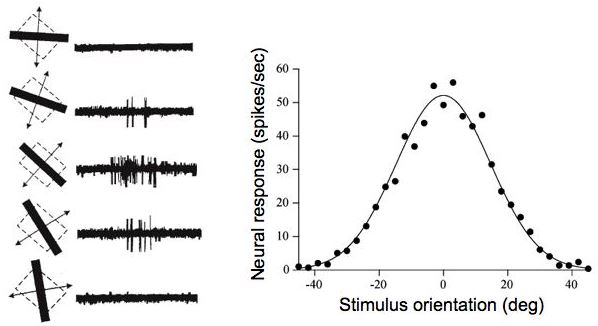
\includegraphics[width=0.8\textwidth]{pics_snn/v1.jpg}
	\caption{Example of rate coding: spike trains for different stimulus orientation (left) of a V1 simple cell of a cat, and the tuning curve (firing rate against stimulus orientation) of the neuron (right)~\cite{hubel1962receptive}.
	The square indicates the visual receptive field of the neuron, and a bar places at different orientation and moves orthogonally is the stimulus.
    As the stimulus becomes more suitable to the preferred orientation ($0^\circ$) of the neuron, the firing rate increases.}
	\label{Fig:v1}
\end{figure}

Rate coding works well when the stimulus is changing slowly and the observation time period is long enough to estimate the firing rate, however in practice the stimulus, e.g. visual sensory input, varies in a fast time scale and the neurons respond within a short reaction time.
Thus, temporal coding is a candidate method to compensate the encoding of fast changing stimulus.

Sound localisation requires temporal coding under precision of milliseconds, which is a good example of one of the temporal coding schemes, phase locking.
Figure~\ref{Fig:audio_fibre} shows phase-locked spike trains generated by Inner Hair Cells in the cochlea.
Phase locking forms the basis
of detecting time differences of binaural sound inputs.
\begin{figure}[bt]
	\centering
	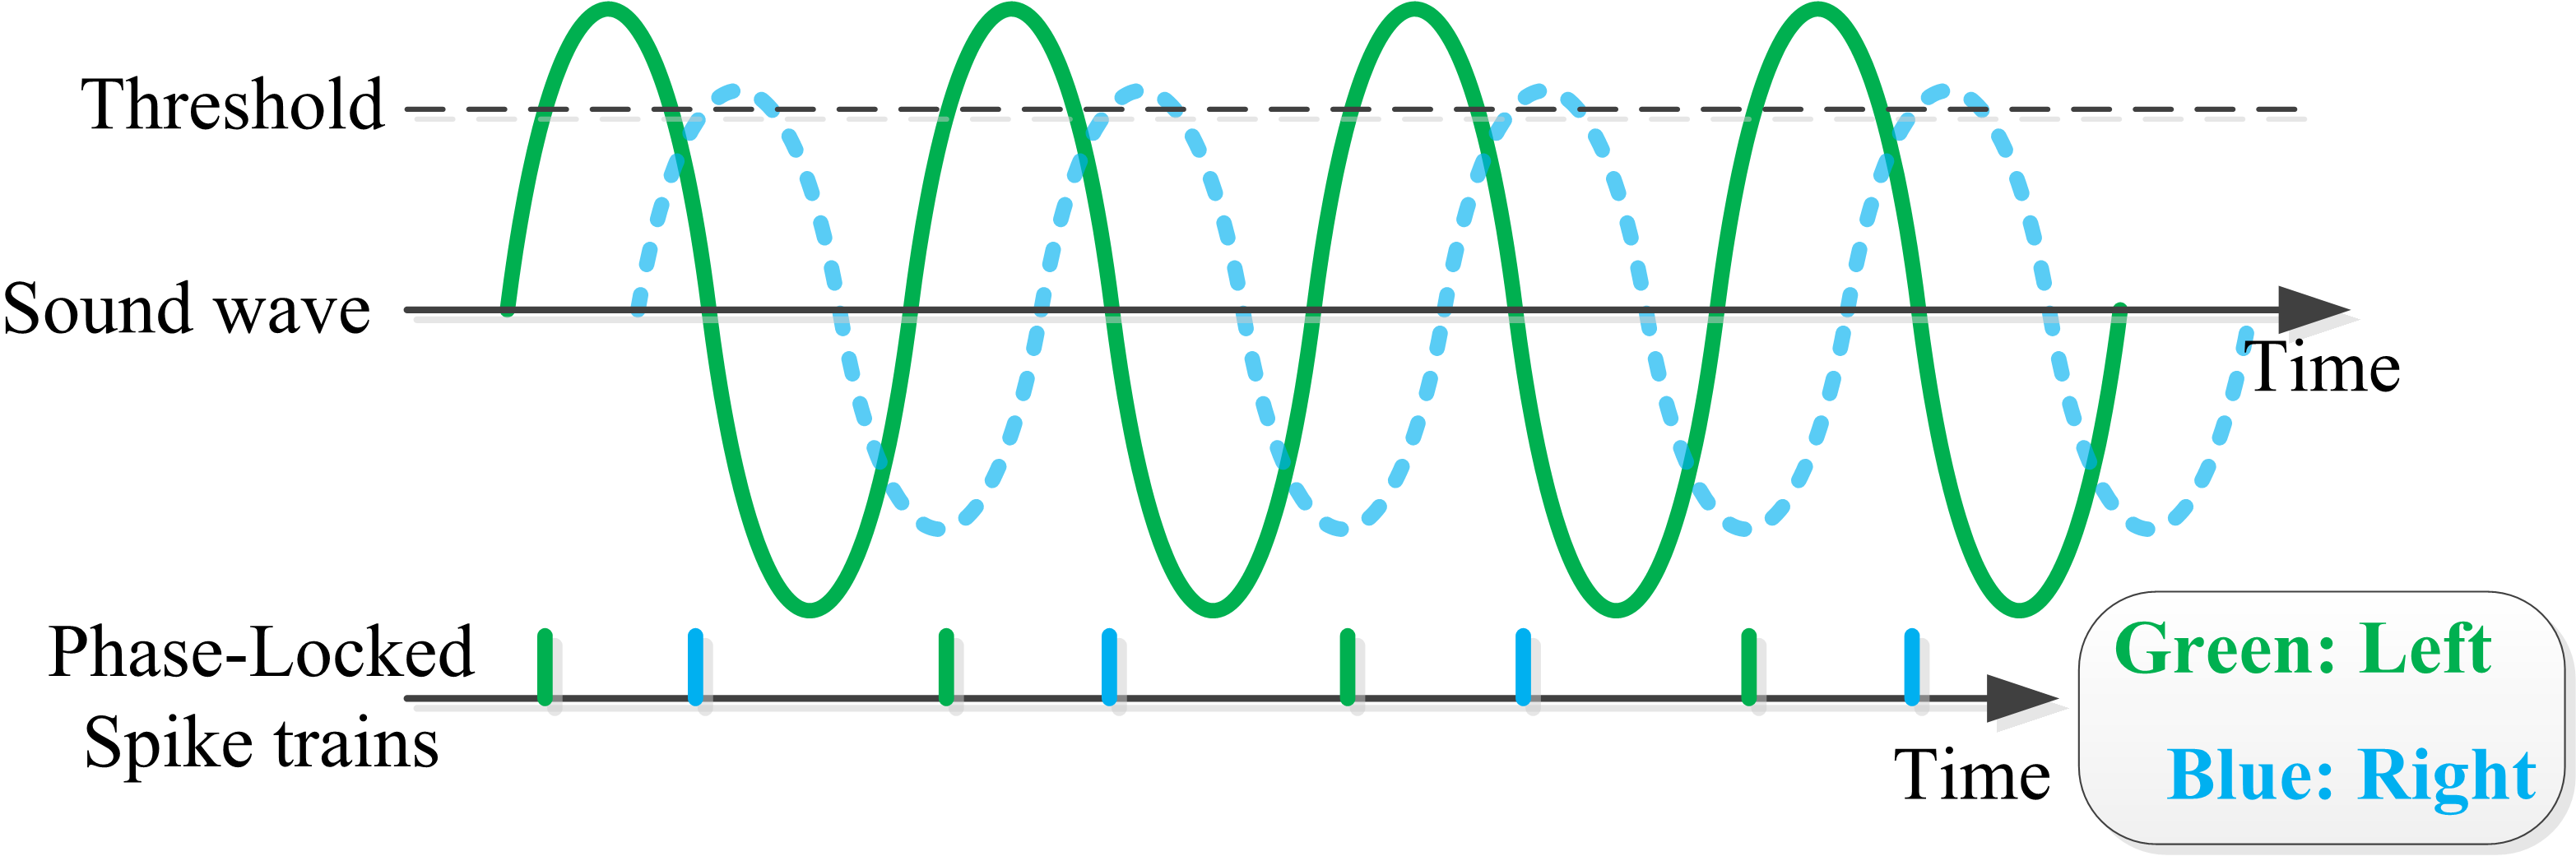
\includegraphics[width=0.8\textwidth]{pics_snn/phaselocking.png}
	\caption{Example of temporal coding: phase-locked spike trains generated by Inner Hair Cells in the cochlea~\cite{liu2013modeling}.
	A sound source generates a sine wave of a certain frequency and conducts to two ears with a time difference and different amplitude due to the angle and distance of the sound source to the head.
	Two spike trains respond to different phases manipulated by a threshold of the sound waves.
	Sound localisation should be resolved by calculating the time difference and level difference of these sound waves which are encoded in the spike trains.
    }
	\label{Fig:audio_fibre}
\end{figure}

Time-to-first-spike encodes the information according to the intensity of a stimulus where a spike shortly after a reference signal indicates a strong stimulation and a later action potential is interpreted as a weaker input.
The tactile afferent information generated by forcing fingerprints from various directions are encoded in such a time-to-first-spike coding scheme~\cite{johansson2004first}.
Synchrony coding also can be found in the brain, where neurons represent the same ``concept'' always fire at the same time~\cite{von1994correlation}, for example in object recognition~\cite{gray1989stimulus}.
Established from the context of fast object recognition, rank-order coding was proposed that it discarded the precise time of spikes, but rather used the relative order of spikes among a group of neurons~\cite{gautrais1998rate}.


\subsection{Signal Transmission}
\label{subsec:spike_trans}
The spike, as an electrical signal, propagates to another neuron at the junction between these two neurons, a chemical synapse.
The axon terminal of a pre-synaptic neuron approaches very close (about 20~nm) to the dendrites (or cell body) of a  post-synaptic neuron.
The tiny space between neurons at a synapse is called the synaptic cleft, which is demonstrated in Figure~\ref{Fig:neuron_basic}(b).
At such a chemical synapse, the action potential generated by the pre-synaptic neuron triggers chemical neurotransmitter molecules to release into the synaptic cleft, and once the post-synaptic neuron detects these neurotransmitters it opens specific ion channels to drive electrical current flowing in.
Hence, synapses completes the transformation from electrical signal to chemical molecules and then back to ion influx.
The amount of neurotransmitters determines how strong the current flows into the post-synaptic neuron.
Thanks to the synaptic plasticity, changes of chemical synapses enables modulations on the synaptic efficacy, and forms the neuronal correlate of learning and memory.

\section{Modelling Spiking Neurons}
\label{sec:spike}
\subsection{Neural Dynamics}
%\subsubsection{Membrane Potential}
The effect of an ion influx on the post-synaptic neuron caused by spike transmission is the change of potential difference across the cell membrane.
This potential difference between the interior and exterior of the cell body, is called the \textbf{membrane potential}.
The membrane potential of a post-synaptic neuron stays at a \textbf{resting potential}, when no input comes.
As soon as a spike arrives, the membrane potential will be either depolarised (increased) or hyper-polarised (decreased) according to the type of synapses, and go back to the resting potential at last.
The behaviour of the membrane potential change caused by a single spike is called the post-synaptic potential (\textbf{PSP}). 
Thus, a spike transmitted by an excitatory synapse triggers an positive change of PSP, named excitatory post-synaptic potential (\textbf{EPSP}), see Figure~\ref{Fig:psp}(a), conversely the negative change, inhibitory post-synaptic potential (\textbf{IPSP}), is driven by inhibitory synaptic event and shown in Figure~\ref{Fig:psp}(b).


%\begin{figure}[tbh!]
%	\centering
%	\begin{subfigure}[t]{0.8\textwidth}
%		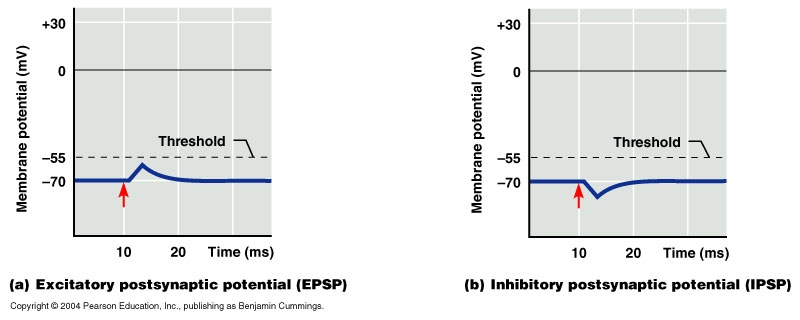
\includegraphics[width=\textwidth]{pics_snn/EI_PSP.JPG}
%		\caption{An electrode measures the \textbf{membrane potential} of a post-synaptic neuron which connected by two pre-synaptic neurons.}
%	\end{subfigure}\\
%	\begin{subfigure}[t]{0.8\textwidth}
%		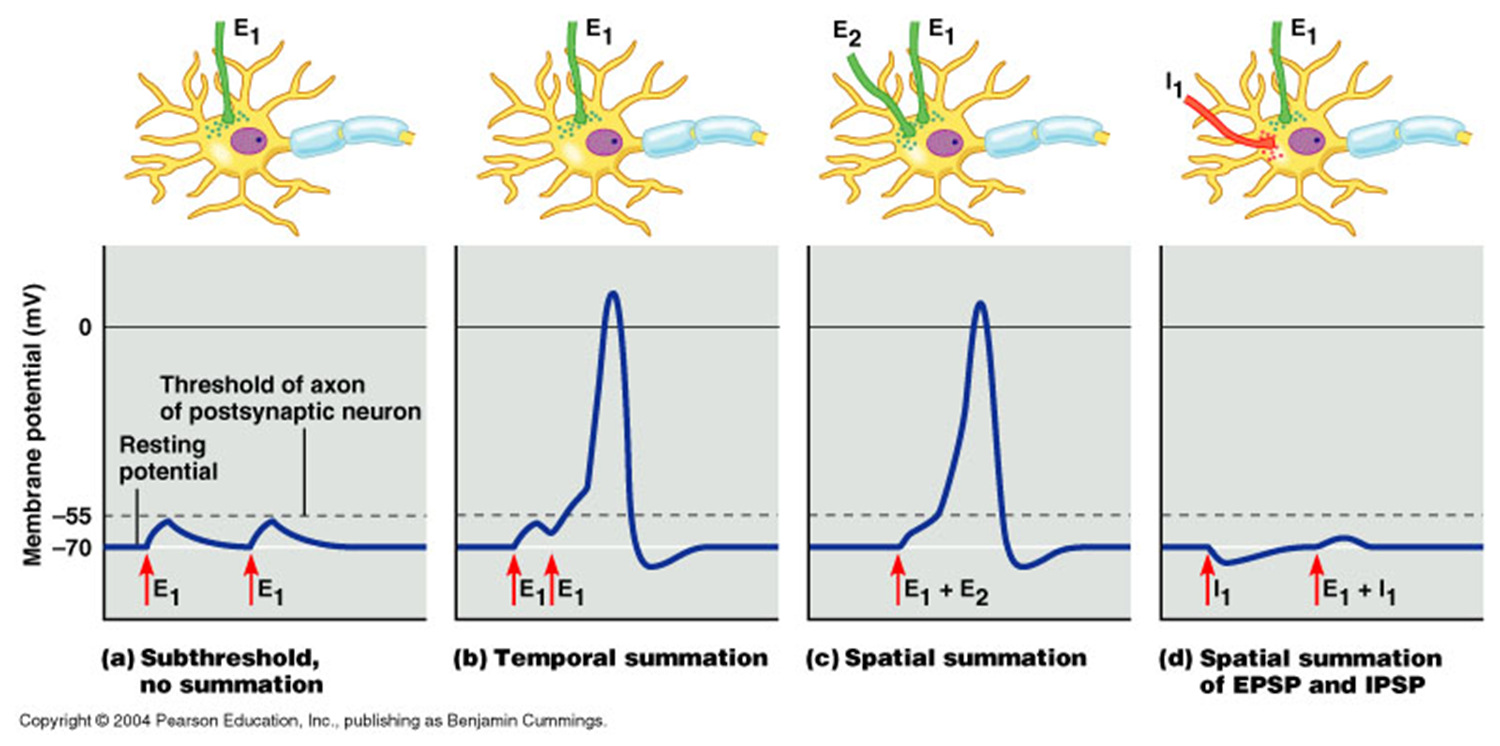
\includegraphics[width=\textwidth]{pics_snn/psp.png}
%		\caption{\textbf{post-synaptic potential (PSP)} generated by spikes of its pre-synaptic neurons adds up to its \textbf{membrane potential} change. }
%	\end{subfigure}
%	\caption{A post-synaptic neuron $i$ receives input from two pre-synaptic neurons $j=1,2$.}
%	\label{Fig:neural_dynamics}
%\end{figure}

\begin{figure}[tb!]
	\centering
	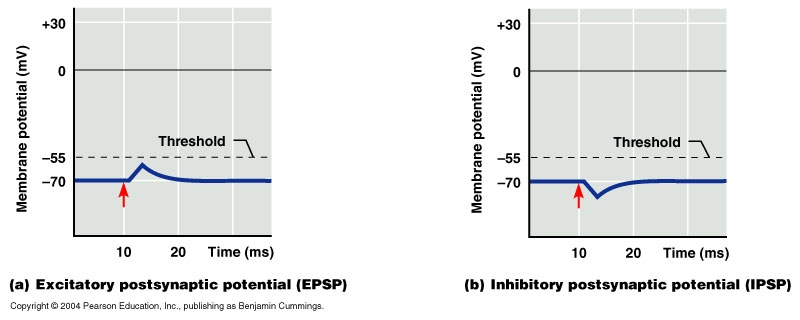
\includegraphics[width=0.9\textwidth]{pics_snn/EI_PSP.JPG}
	\caption{Post-synaptic potential driven by a spike, where the red arrow represents a spike arriving at the neuron~\cite{marieb2007human}.}
	\label{Fig:psp}
\end{figure}

\begin{figure}[bt!]
	\centering
	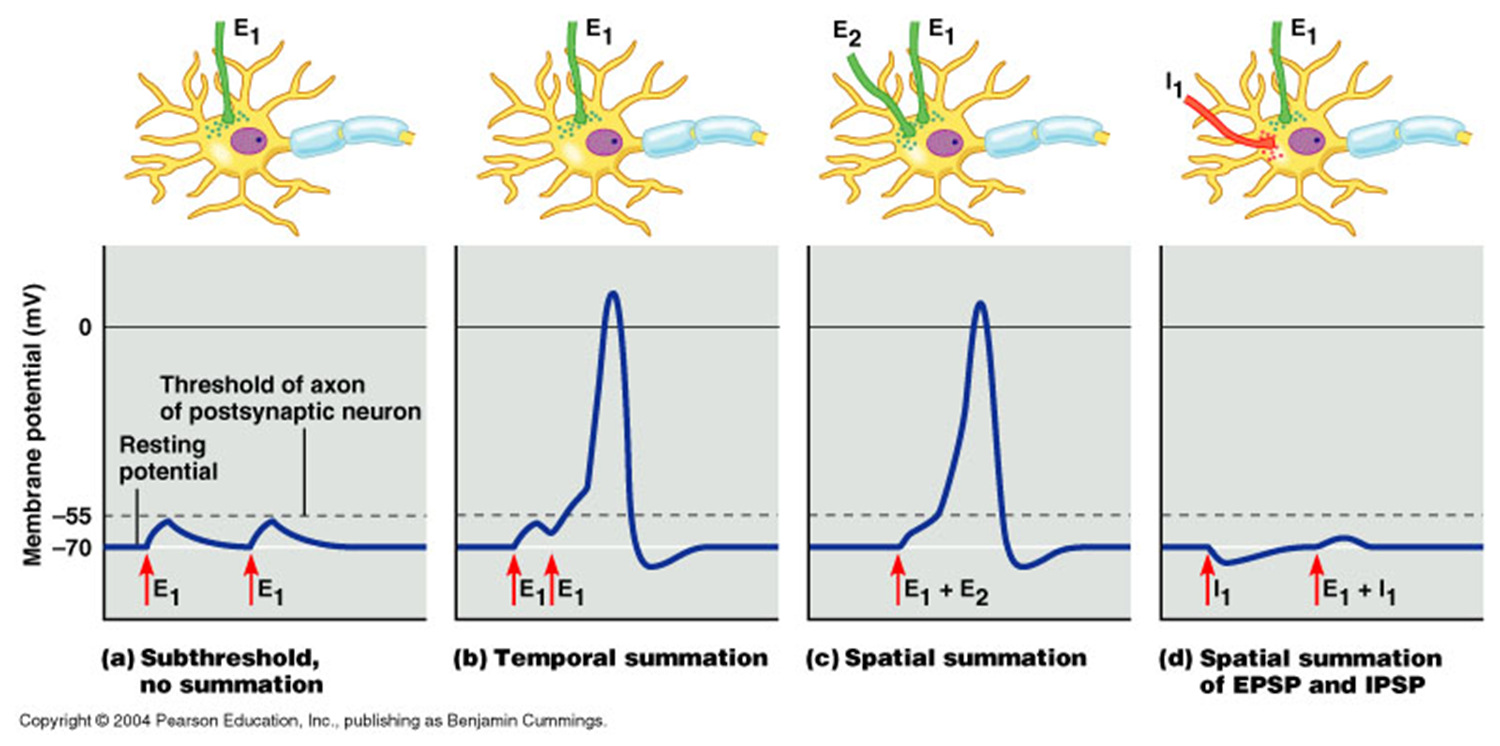
\includegraphics[width=0.9\textwidth]{pics_snn/psp.png}
	\caption{Summation of post-synaptic potentials~\cite{reece2011campbell}. 
		(a) Single EPSPs are usually not strong enough to trigger an action potential without summation. (b) Temporal summation of two EPSPs of the same synapse generates an action potential. (c) Spatial summation of two EPSPs of two synapse generates an action potential. (d) Spatial-temporal summation of both EPSP and IPSPs.
	}
	\label{Fig:psp_sum}
\end{figure}

Singe PSPs have an accumulated effect on the membrane potential both in temporal and spatial.
The accumulation performs simple summation of PSPs until the membrane potential reaches a \textbf{threshold}, that an action potential will be generated at the post-synaptic neuron.
Figure~\ref{Fig:psp_sum} illustrates temporal and spatial summations of PSPs under different circumstances.




\subsection{Neuron Models}
The keys of modelling a spiking neuron are: 
\begin{itemize}
	\item to mathematically formalise the evolution of membrane potential;
	\item to states a mechanism of spike generation.
\end{itemize}

\subsubsection{Leaky Integrate-and-Fire}
\begin{figure}[tb!]
	\centering
	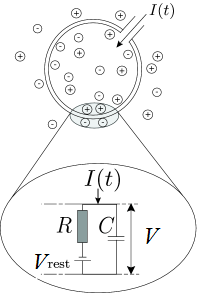
\includegraphics[width=0.3\textwidth]{pics_snn/RC.png}
	\caption{Current flowing into a neuron functions like a resistor–capacitor (RC) circuit~\cite{gerstner2014neuronal}.}
	\label{Fig:rc}
\end{figure}

The evolution of membrane potential can be simplified as a resistor–capacitor (RC) circuit which consists of a membrane capacitor, $C_m$ and a membrane resistance $R_m$, both driven by input current flow $I$, see Figure~\ref{Fig:rc}.
In the resting state without any input, the membrane potential $V$ stays at the same potential as the battery $V_{rest}$.
When current flows into the neuron, it will charge the capacitor $I_C(t)$ and flow through the resistance $I_R(t)$ to depolarise the membrane potential when the current stops the capacity charge will decay back to $V_{rest}$ by leaking through the resistance:
\begin{equation}
\begin{aligned}
	I(t) &= I_R(t) + I_C(t) \\[10pt]
	&= \dfrac{V-V_{rest}}{R_m} + C_m \dfrac{\D V}{\D t}~~.
\end{aligned}
\label{equ:LIF_current}
\end{equation}
The standard form of the LIF model describes the sub-threshold membrane potential evolution:
\begin{equation}
	\tau_m \dfrac{\D V}{\D t} = -(V-V_{rest}) + R_m I(t)~,
\end{equation}
where $\tau_m = C_m R_m$ is called the membrane time constant, and as soon as the membrane potential reaches the threshold $V_{thresh}$, it is set to a reset potential $V_{reset}$, which is usually lower than $V_{rest}$: 
\begin{equation}
V = V_{reset}~.
\end{equation}
The simple LIF model uses: (1) a linear differential equation to describe the evolution of membrane potential;
and (2) a threshold to generate a spike .

\subsubsection{Hodgkin-Huxley}
Hodgkin-Huxley is the Nobel Prize winning model that explains ionic mechanisms generating and transmitting action potentials in the squid giant axon~\cite{hodgkin1939action}.
The current $I_R(t)$ which flows through the membrane resistance is determined by three ion channels: a leak channel with a conductance of $g_L$, the sodium channel of $g_{Na}$ conductance and the potassium channel of  $g_{K}$ conductance.
The currents flow through these channels are all proportional to the difference between the membrane potential and the reversal potentials of the channels: $V-E_L$, $V-E_{Na}$, and $V-E_{K}$ respectively.
Thus Equation~\ref{equ:LIF_current} is detailed as:
\begin{equation}
\begin{aligned}
I(t) &= I_L(t) + I_{Na}(t) + I_{K}(t)+ I_C(t) \\
&= g_L(V-E_L) + g_{Na}m^3h(V-E_{Na}) + g_{K}n^4(V-E_{K})  + C_m \dfrac{\D V}{\D t}~~.
\end{aligned}
\label{equ:HH_current}
\end{equation}
 
The Hodgkin–Huxley model can be seen as a non-linear differential equation with four state variables, $V$, $m$, $h$ and $n$ that change against time:
\begin{equation}
\begin{aligned}
C_m \dfrac{\D V}{\D t} = I(t) - g_{K}n^4(V-E_{K}) &- g_{Na}m^3h(V-E_{Na}) - g_L(V-E_L)~, \textrm{~~and }\\[10pt]
\dfrac{\D m}{\D t} &= \alpha_m(V)(1-m) - \beta_m(V)m~, \\[10pt]
\dfrac{\D n}{\D t} &= \alpha_n(V)(1-n) - \beta_n(V)n~, \\[10pt]
\dfrac{\D h}{\D t} &= \alpha_h(V)(1-h) - \beta_h(V)h~,
\end{aligned}
\end{equation} 
where $\alpha(V)$ and  $\beta(V)$ are empirical functions of membrane potential.
Regarding to the mechanism of spike initiation, it refers to the most significant property of the Hodgkin-Huxley model that the model is able to generate action potentials with the changes of those dynamic internal variables alone.

The Hodgkin-Huxley equations provides a detailed, quantitative, and reasonable accurate mathematical model explaining the evolution of the membrane potential and the action potential~\cite{byrne2014molecules}.
However, its numerical complexity and highly non-linearity prohibit it from being intuitively understood and make large-scale simulations too expensive.
Therefore, neural model selection should take account of objectives, degree of detail and computational power.

\subsubsection{Izhikevich}
Izhikevich model is proposed to solve the problems of computational complexity of the Hodgkin-Huxley model and the insufficient capability of LIF model for reproducing complex dynamics of cortical neurons~\cite{izhikevich2003simple}.
Thus the model can be employed to simulate large-scale brain models consisted of real biological neurons.

The membrane potential evolves in accordance with a pair of differential equations:
\begin{equation}
\begin{aligned}
\dfrac{\D v}{\D t} &= 0.04v^2 + 5v + 140 - u - I(t)~,\\[10pt]
\dfrac{\D u}{\D t} &= a(bv - u)~,
\end{aligned}
\end{equation}
where $v$ is the membrane potential and $u$ represents the membrane recovery which negatively feeds back to $v$.
In terms of spike generation, the initiation part of an activation potential is produced by the equations, but a resetting scheme is needed:
\begin{equation}
\left\{
\begin{aligned}
v &= c \\
u &= u + d
\end{aligned}
\right.
\textrm{~~~~when~} v \geq 30.
\end{equation}  
$a$, $b$, $c$, and $d$ are constant parameters that can be configured to reproduce various neural dynamics of real biological neurons~\cite{izhikevich2004model}.

\subsection{Synapse Model}
Applying spiking neuron models to synaptic spike transmissions, we can use two types of synapses: current-based and conductance-based models.
Thus the synaptic efficacy $w$ determines either the input current intensity flowing through the synapse: % (current-based model)
\begin{equation}
I(t) = w(t)~,
\end{equation}
or the electric conductance $g_{syn}$ of the ion channel: % (conductance-based model)
\begin{equation}
I(t) = g_{syn} (V-E_{syn}) = w(t) (V-E_{syn})~,
\end{equation}
where $E_{syn}$ indicates the reversal potential of a synapse.
Both equations identify the strength of a synaptic current, thus simply adding up all the synaptic currents on the same post-synaptic neuron that the summation can be picked up as the external current by all the neuron models stated above.
%\begin{equation}
%I(t) = \sum_j I_{ij}(t)~.
%\end{equation}

The current flow usually takes much longer than an action potential and decays over time, thus an simple exponential decay is able to model the decaying synaptic efficacy.
Assuming spikes are delivered at time $t={t_0, t_1, ..., t_n}$, the initial synaptic weight is set to $w_0$ and $\tau_{syn}$ is the synaptic time constant, the decaying synaptic current or the conductance can be described as:
\begin{equation}
w(t) = \sum_k w_0 \exp^{-(t-t_k)/\tau_{syn}}~.
\end{equation}

In the thesis we mostly employ LIF neurons and current-based synapse model with decaying synaptic efficacy, thanks to its simple mathematical expression, low numerical complexity and high-level abstraction that hiding much of detailed neural dynamics.
Therefore, at the initial stage of merging artificial deep learning to biologcial-plausible SNNs, we can (1) analytically solve the linear differential equation thus to understand and to use the LIF model well; (2) simulate large-scale SNN with deep architectures without a tight limitation on computational power; and (3) have much fewer parameters to concern about resulting in a simplified problem.


\subsection{Synaptic Plasticity}
As mentioned in Section~\ref{subsec:spike_trans}, synaptic plasticity forms the neuronal level of learning and memory of the brain.
%This synaptic plasticity was firstly proved by Bliss and L{\o}mo that if two neurons fired simultaneously then their synaptic connection would be strengthened~\ref{bliss1973long}.
Biological observations have provided evidence that modulations on the synaptic efficacy depend on the relative timing of the pre- and post-synaptic spikes\cite{bi2001synaptic}.
This mechanism is known as synaptic time-dependant plasticity (\textbf{STDP})~\cite{gerstner1996neuronal}.

\begin{figure}[bt]
	\centering
	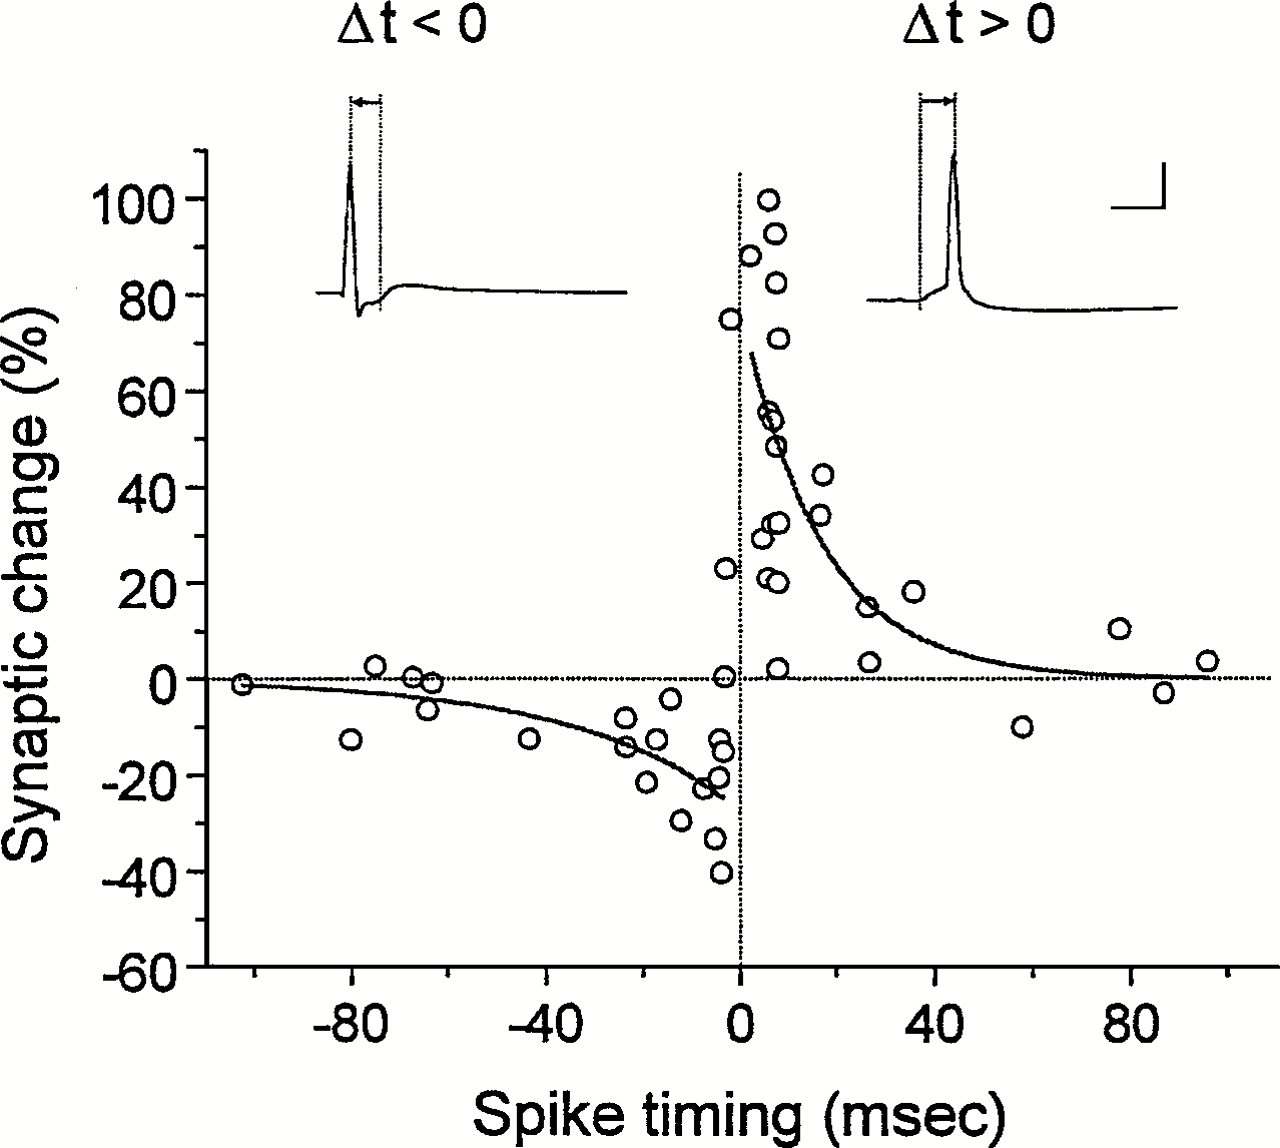
\includegraphics[width=0.5\textwidth]{pics_snn/stdp.jpeg}
	\caption{Synaptic time dependant plasticity~\cite{bi2001synaptic}.}
	\label{Fig:STDP}
\end{figure}

When a presynaptic spike
arrives before a postsynaptic spike is emitted the synapse is potentiated (strength-
ened). However, if a presynaptic spikes arrives after a postsynaptic spike has been
emitted, the synapse is depressed (weakened). Furthermore the data recorded by
Bi and Poo suggest that the magnitude of the changes in synaptic efficacy (∆w i j )
is related to the relative spike timings with the following exponential functions




\section{Simulating Networks of Spiking Neurons}
\label{sec:snn_sim}
\subsection{Software Simulators}
clock driven

event driven

hybrid simulators Brian, Nest and Neuron

PyNN
\subsection{Neuromorphic Hardware}
Table from Steve
\subsection{Neuromorphic Standing-alone Systems}
Papers listed.
Vision and Auditory
\label{sec:morph}

